\chapter{Fractures}

\begin{figure}[h!]
    \centering
    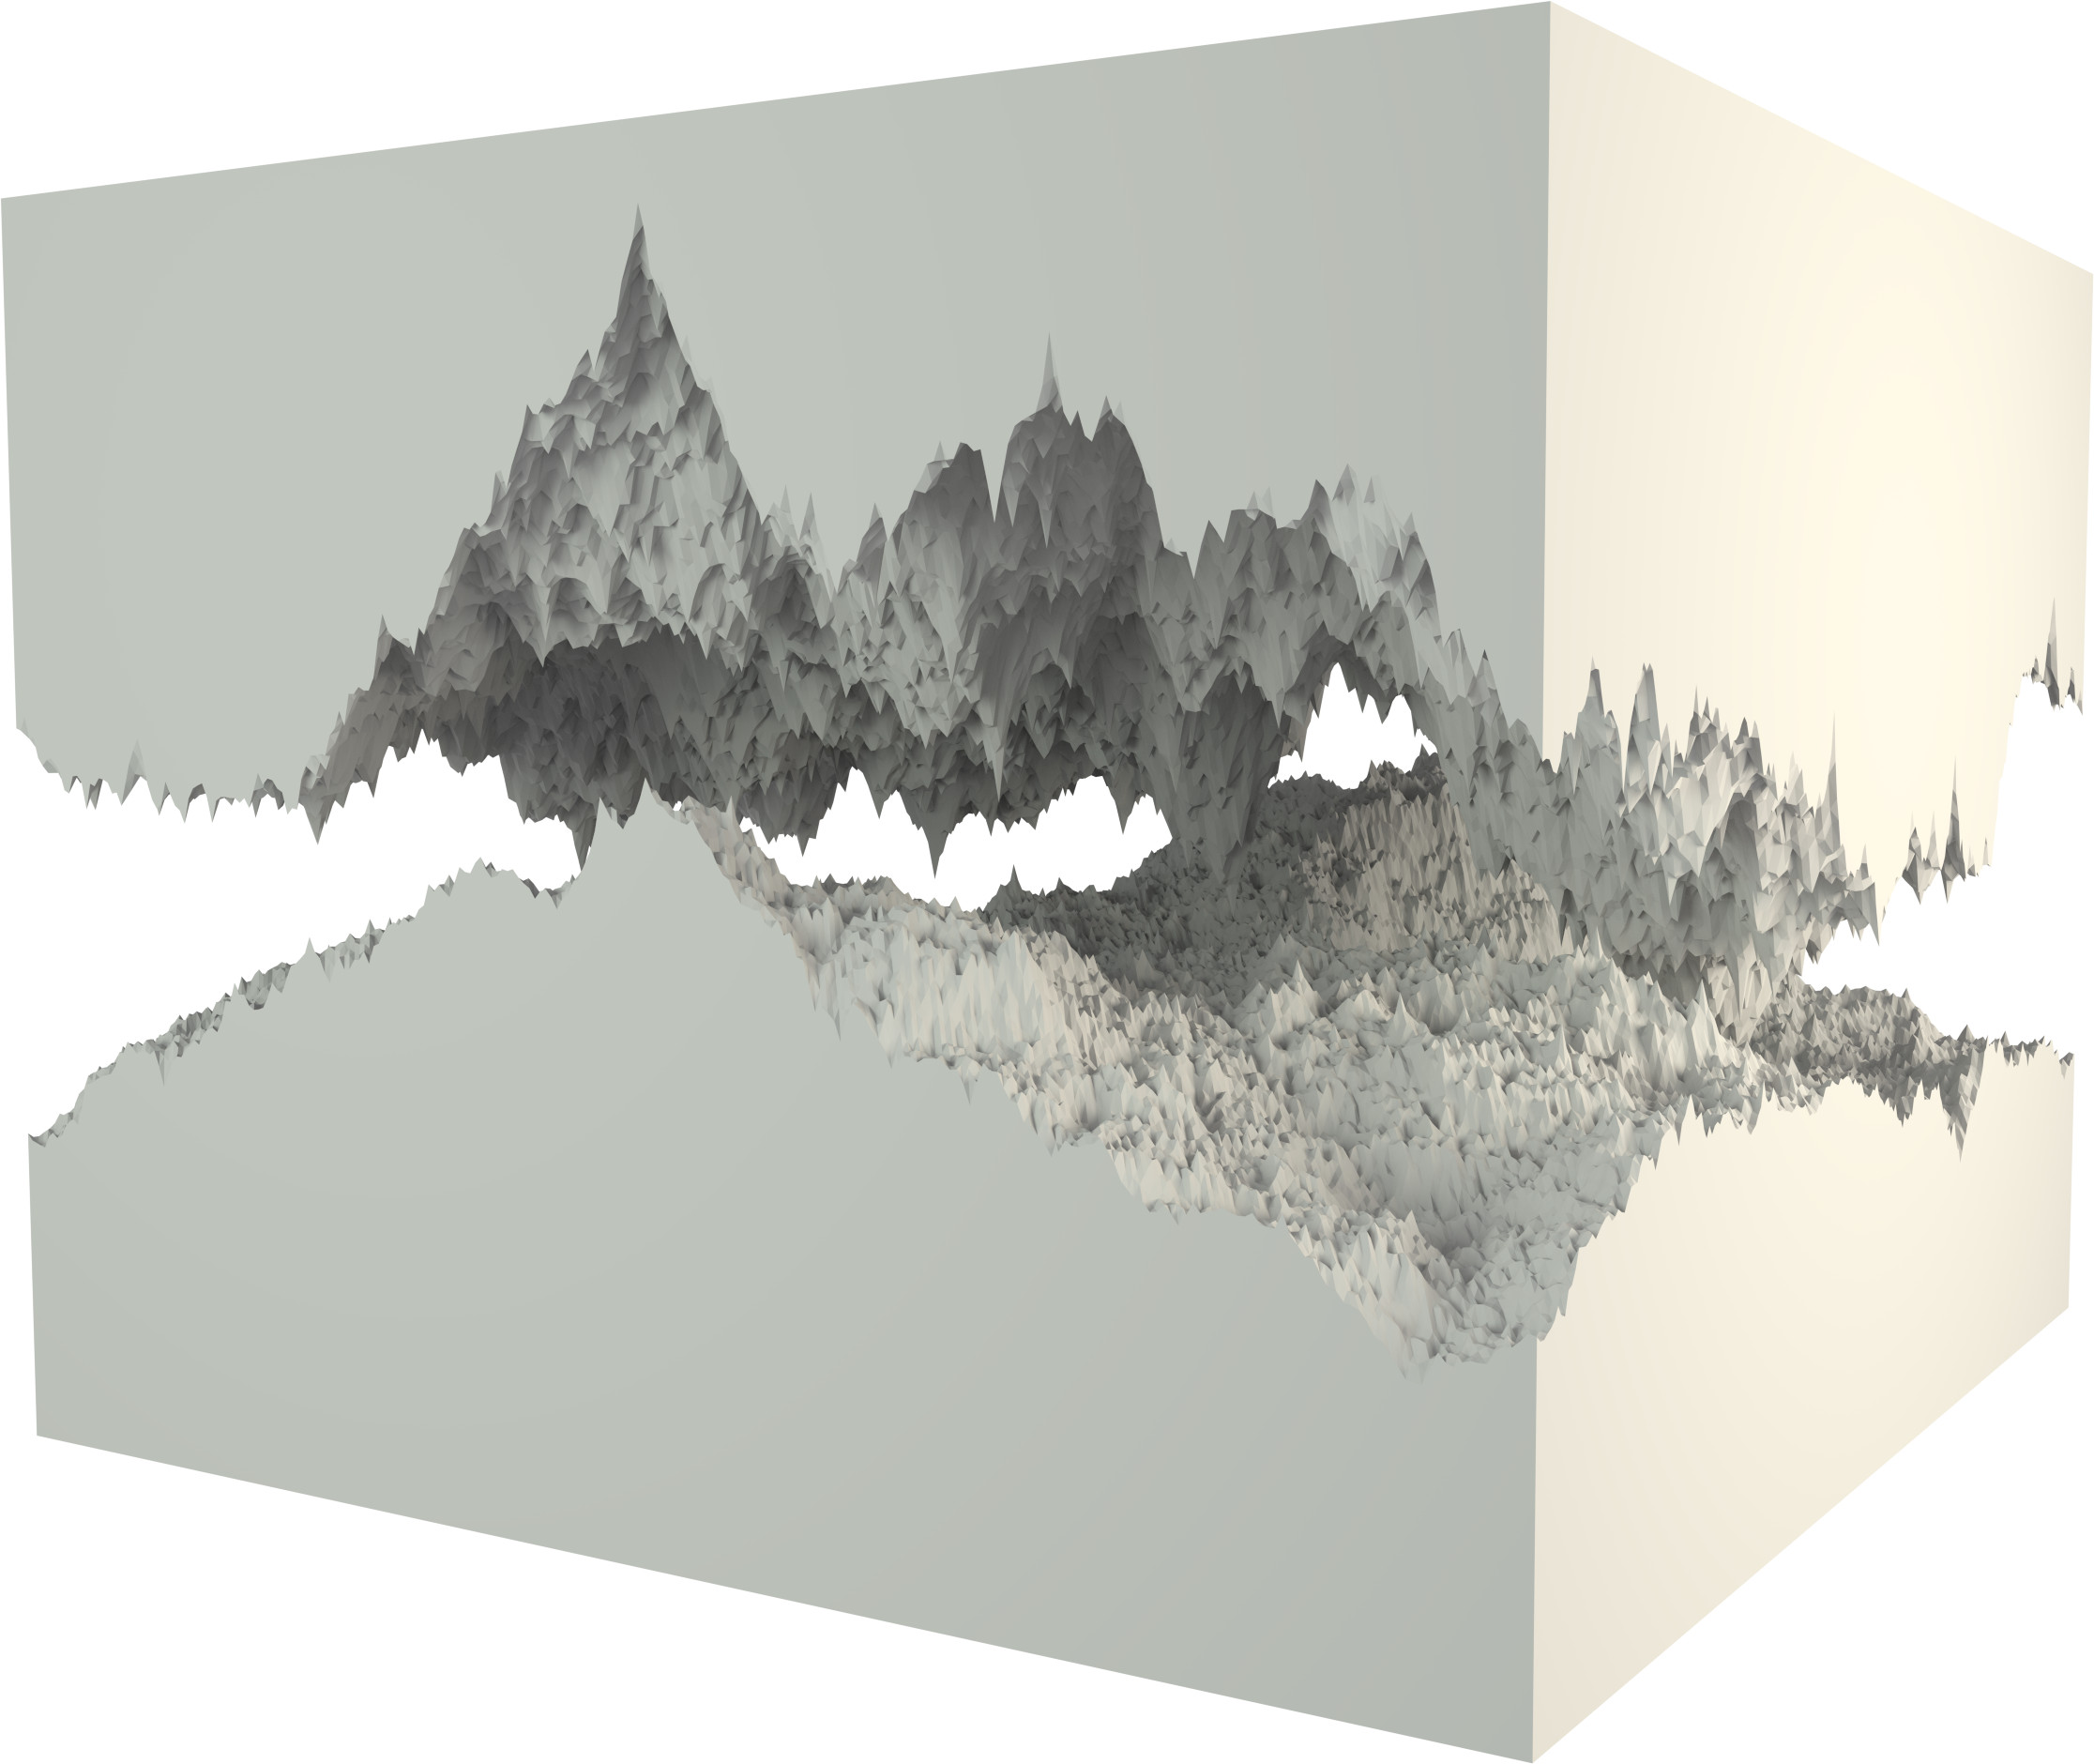
\includegraphics[width=\textwidth]{images/fracture/large_fracture05.jpg}
    \caption{Caption}
\end{figure}

We want to study the behaviour of water trapped in nanoscale (pores and) fractures in silica, so need want a way to generate and characterize such a structure. (Several methods of characterizing a fracture could be imagined (\hl{SOURCES, examples}), and we will use several of them.)        

\hl{terrain == heightmap??, finn bra ord her}

\section{Characterization}

\todo{change wording? copied from Fractals...}
An \emph{affine transformation} transforms a point $\bvec x = (x_1, \dots, x_n)$ into new points $\bvec x' = (r_1x_1, \dots, r_n, x_n)$, where the scaling rations $r_1, \dots, r_n$ are \emph{not} all equal.

A bounded set $\mathcal{S}$ is \emph{self-affine} if $\mathcal{S}$ is the union of $N$ non-overlapping subsets $\mathcal{S}_1, \dots, \mathcal{S}_N$, each of which is congruent to the set $\bvec r(\mathcal{S})$ obtained from $\mathcal S$ by the affine transform defined by $\bvec r$. Here \emph{congruent} means that the set of points $\mathcal{S}$ is identical to the set of points $\bvec r(\mathcal{S})$ after possible translations and/or rotations of the set\cite{feder1988fractals}.

A set $\mathcal{S}$ is \emph{statistically self-affine} if $\mathcal{S}$ is the union of $N$ non-overlapping subsets each of which is scaled down by $\bvec r$ from the original, and is identical in all statistical respects to $\bvec r(\mathcal{S})$.

\subsection{Hurst exponent}
\orangebox{
\begin{itemize}
    \item define fractal dimension
\end{itemize}
}

To characterize a fractal one can use the Hurst exponent, usually called $H$\footnote{\todo[inline]{The name used by Hurst in his work where he first describes the exponent was actually $K$\cite{hurst1965longterm}\cite{hurst1951longterm}}}, which comes from a statistical method developed by Hurst\cite{hurst1965longterm}\cite{hurst1951longterm}. The Hurst exponent is related to the fractal dimension $D$ by
\begin{align*}
    D = d-H,
\end{align*}
where $d$ is the spatial dimension of the fractal's domain\cite{feder1988fractals}.

The statistical method developed by Hurst is called \emph{rescaled range analysis} and was designed for use on 1-dimensional time series $f(t)$. The method has been generalized to higher dimensions\cite{fan2013rescaled}, but the original 1D form is shown here.

\subsubsection{Rescaled range analysis}
First the time series is divided into \todo{overlapping/non-overlapping?} intervals of length $\tau$. The average over each interval of length $\tau$ is
\begin{align*}
    \langle f \rangle_\tau = \frac{1}{\tau} \sum_{t=1}^\tau f(t).
\end{align*}
We let $F$ be the accumulated deviation from the mean
\begin{align*}
    F(t, \tau) = \sum_{t' = 1}^t \big( f(t') - \langle f \rangle_\tau \big).
\end{align*}
The difference between the maximum and minimum of the accumulated deviation from the mean is the \emph{range} R
\begin{align*}
    R(\tau) = \max_{1 \leq t \leq \tau} \big(F(t,\tau)\big) - \min_{1 \leq t \leq \tau} \big(F(t, \tau)\big).
\end{align*}
The standard deviation $S$ of the time series is estimated using
\begin{align*}
    S^2 = \frac{1}{\tau} \sum_{t=1}^\tau \big( f(t) - \langle f \rangle_\tau \big)^2.
\end{align*}
Hurst found that the observed \emph{rescaled range}, $R/S$, for many time series is described by the \hl{empirical} relation\cite{feder1988fractals}
\begin{align*}
    \frac{R}{S} = \left(\frac{\tau}{2}\right)^H \sim \tau^H.
\end{align*}
We now see that we can estimate the Hurst exponent by a linear fit of the form
\begin{align*}
    \log \left(\frac{R}{S}\right) \sim H\log\tau,
\end{align*}
where we find $H$ as the slope of the linear fit.

\todo[inline]{Something about that it's hard to measure, and why.}

\subsubsection{Detrending moving average}
To estimate the Hurst exponent of a surface we use a method called detrending moving average (DMA) first described by E. Alessio, A. Carbone et al.\cite{alessio2002dma}, and later generalized to higher dimensions by A. Carbone \cite{carbone2007algorithm}. We use this method because ??? \todo[inline]{good results, easy to implement? }

We define a \hl(self-affine) surface as $f(i,j)$, where $f$ is the height in the point $(i,j)$, defined in a discrete 2-dimensional domain with size $N\times N$, and with $i,j = 1,\dots,N$. We divide the surface into square \hl{subsurfaces} of size $n \times n$, and find the average $\tilde f_n$ of each subsurface by\footnote{\cref{eq:carbone_average} is how the average $\tilde f_n$ is stated in the article\cite{carbone2007algorithm}, but we rewrite it to \cref{eq:carbone_average_rewritten} so it's easier to understand. The two forms are equivalent.}
\begin{align}
    \tilde f_n(i,j) 
    &= \frac{1}{n^2}\sum_{k=-m}^{n-1-m} ~ \sum_{l=-m}^{n-1-m} f(i-k, j-l) \label{eq:carbone_average}\\
%     &= \frac{1}{n^2}\sum_{k=i-m}^{i-n+1+m}\sum_{l=j-m}^{j-n+1+m} f(i-k, j-l) \\
    &= \frac{1}{n^2} \sum_{k=(i+m)-n+1}^{i+m} ~ \sum_{l=(i+m)-n+1}^{i+m} f(k, l), \label{eq:carbone_average_rewritten}
\end{align}
where
\begin{align*}
    &m = \left \lfloor n\theta \right \rfloor &\text{for }0 \leq \theta < 1,
\end{align*}
which means that $0 \leq m \leq (n-1)$. $\theta$ is a parameter that controls the position of the square relative to the point $(i,j)$ in $\tilde f_n(i,j)$. There are three \hl{extreme} cases for $\theta$, which are listed below, and are illustrated in \cref{fig:DMA_theta}.
% \begin{itemize}
%     \item For $\theta = 0$ we have $m=0$ and we average over a square with the point $(i,j)$ in the square's upper right corner (($i-n+1) \leq k,l \leq i$). See \cref{fig:DMA_theta_a}.
%     \item For $\theta = 1/2$ we average over a square centered on the point $(i,j)$. See \cref{fig:DMA_theta_b}.
%     \item For $\theta = (n-1)/n$ we have the maximum value for $m$, $m=n-1$, and average over a square with the point $(i,j)$ in the square's lower left corner \todo{THESE LIMITS ARE WRONG??}($i \leq k,l \leq (i+n-1)$). See \cref{fig:DMA_theta_c}.
% \end{itemize}
\begin{description}
    \item[$\bm{\theta = 0}$:] \hfill\\ 
        We have $m=0$ and we average over a square with the point $(i,j)$ in the square's upper right corner (($i-n+1) \leq k,l \leq i$). See \cref{fig:DMA_theta_a}.
    \item[$\bm{\theta = 1/2}$:] \hfill\\ 
        We average over a square centered on the point $(i,j)$. See \cref{fig:DMA_theta_b}.
    \item[$\bm{\theta = (n-1)/n}$:] \hfill\\ 
        {\sloppy 
        We have the maximum value for $m$, $m=n-1$, and average over a square with the point $(i,j)$ in the square's lower left corner \todo{\st{THESE LIMITS ARE WRONG??} fixed}\\(${i \leq k,l \leq (i+n-1)}$). See \cref{fig:DMA_theta_c}.
        }
\end{description}

\begin{figure}
    \centering
    \begin{subfigure}[b]{0.25\textwidth}
        \includesvg[width=\textwidth, svgpath=./images/Hurst/]{2DDMA_theta04_a}
%         \caption{Illustration of how to divide a convex hexahedron into five tetraheda.}
        \caption{$\theta = 0$}
        \label{fig:DMA_theta_a}
    \end{subfigure}
    \hspace{0.1\textwidth}
    \begin{subfigure}[b]{0.25\textwidth}
        \includesvg[width=\textwidth, svgpath=./images/Hurst/]{2DDMA_theta04_b}
%         \caption{A random fracture made from two periodic heightmaps.}
        \caption{$\theta = 1/2$}
        \label{fig:DMA_theta_b}
    \end{subfigure}
    \hspace{0.1\textwidth}
    \begin{subfigure}[b]{0.25\textwidth}
        \includesvg[width=\textwidth, svgpath=./images/Hurst/]{2DDMA_theta04_c}
%         \caption{A random fracture made from two periodic heightmaps.}
%         \caption{$\theta \rightarrow 1$ \\ ($\theta = (n-1)/n$)}
%         \caption{$\theta \rightarrow 1$}
        \caption{$\theta = (n-1)/n$}
        \label{fig:DMA_theta_c}
    \end{subfigure}
        \caption{
        Illustration of what the parameter $\theta$ controls in the detrending moving average method in 2 dimensions. The circles are points where the surface is defined, the red star is the point $(i,j)$, and the black square encompasses the points averaged over to calculate $\tilde f_n(i,j)$ in \cref{eq:carbone_average_rewritten}. The illustration uses $n = 3$.
        \label{fig:DMA_theta}
    }
\end{figure}

We then define the generalized variance $\sigma_\text{DMA}^2$
\begin{align*}
    \sigma_\text{DMA}^2 
    = \frac{1}{(N-n)^2}\sum_{i=n-m}^{N-m} ~ \sum_{j=n-m}^{N-m} 
    \big(
        f(i,j) - \tilde f_n(i,j)
    \big)^2,
\end{align*}
where we see that $f(i,j) - f_n(i,j)$ is the difference between the point $(i,j)$ and the average of a square of points (including the point itself) of size $n \times n$, as explained above (see \cref{fig:DMA_theta}).
% (the position of the square is controlled by the parameter $\theta$, as explained above, and illustrated \cref{fig:DMA_theta}). 
The summation limits $(n-m) \leq i,j \leq N-m$ are set so that the averages $f_n(i,j)$ don't exceed the domain with size $N \times N$.

The generalized variance goes as
\begin{align*}
    \sigma_\text{DMA}^2 \sim \left(2n^2\right)^H,
\end{align*}
which we can use to find the Hurst exponent $H$, by calculating $\sigma_\text{DMA}^2$ for different sizes of the squares, $n$. We estimate $H$ by a linear fit of $\log \sigma_\text{DMA}^2$ against $\log 2n^2$, where $H$ is the slope.

In the paper that generalizes DMA to higher dimensions\cite{carbone2007algorithm} they use different parameters for each spatial dimension $d$, $\bvec\theta = \theta_1, \dots, \theta_d$ and $\bvec{n} = n_1, \dots, n_d$, but for simplicity and to avoid \hl{strange} results, we use $\theta_1 = \theta_2 = \theta$ and $n_1 = n_2 = n$.

% With $\theta = 0$ we have $m = 0$ and average over all points $(\leq k \leq i,l \leq j)$. 

% With $\theta = n/(n-1)$ we have $m = n-1$, and average over all points $(k \geq i,l \geq j)$.

% We define the generalized variance $\sigma_\text{DMA}^2$ as the variance 
% \begin{align*}
%     \sigma_\text{DMA}^2 
%     = \frac{1}{(N-n)^2}\sum_{i=n-m}^{N-m}\sum_{j=n-m}^{N-m} 
%     \big(
%         f(i,j) - \tilde f_n(i,j)
%     \big)^2,
% \end{align*}
% where\footnote{We rewrite \cref{eq:carbone_average} for easier understanding}
% \begin{align}
%     \tilde f_n(i,j) 
%     &= \frac{1}{n^2}\sum_{k=-m}^{n-1-m}\sum_{l=-m}^{n-1-m} f(i-k, j-l) \label{eq:carbone_average}\\
% %     &= \frac{1}{n^2}\sum_{k=i-m}^{i-n+1+m}\sum_{l=j-m}^{j-n+1+m} f(i-k, j-l) \\
%     &= \frac{1}{n^2} \sum_{k=(i+m)-n+1}^{i+m} ~ \sum_{l=(i+m)-n+1}^{i+m} f(k, l).\nonumber %\label{eq:carbone_average_rewritten}
% \end{align}
% \begin{align*}
%     m = \left \lfloor n\theta \right \rfloor
% \end{align*}
% $\theta = 1$ or $\theta = 0$ (directed implementation, for fractals with preferential growth direction) \\
% $\theta = 0.5$ (isotropic implementation, ``uniformity in all orientations'') \\



% \begin{figure}
%     \centering
%     \includesvg[width=0.99\textwidth, svgpath=./images/Hurst/]{2DDMA_theta04}
%     \caption{
%         Illustration of what the parameter $\theta$ controls in the detrending moving average method in 2 dimensions. The circles are points where a surface is defined, the red star marks the point $(i,j)$, and the black square marks the points averaged over to calculate $\tilde f_n(i,j)$ in \cref{eq:carbone_average_rewritten}.
%         \label{fig:DMA_theta}
%     }
% \end{figure}



% \subsubsection{Detrended fluctuation analysis in higher dimensions}
% original DFA\cite{peng1994mosaic}
% HDDMA\cite{gu2006detrended}
% 
% To estimate the Hurst exponent of a fracture we use a generalized version of a method called \emph{detrended fluctuation analysis}\cite{peng1994mosaic}, which was generalized to higher dimensions by Gu and Zhou\cite{gu2006detrended}.
% 
% The two-dimensional DFA:
% 
% We have a self-affine surface stored in the matrix $f(i,j)$, where $f$ \hl{is} the height of the surface in the point $(i,j)$, with $i,j = 1,\dots,N$, and $N^2$ is the number of points where the surface is defined. The surface is divided into $n\times n$ disjoint (non-overlapping) \hl{and neighboring} surfaces \todo{sub-surface?} of the same size $s\times s$, where $n = N/s$. Each of these surfaces is denoted by $f_{u,v}$ such that $f_{u,v}(i,j) = f(i+k, j+l)$ for $i,j = 1, \dots, s$, where $k = (u-1)s$ and $l = (v-1)s$.
% 
% For a surface $f_{u,v}$ the cumulative sum $F_{u,v}(i,j)$ is calculated as follows
% \begin{align*}
%     F_{u,v}(i,j) = \sum_{m=1}^i\sum_{n=1}^j f_{u,v}(m,n),
% \end{align*}
% where $i,j = 1,\dots,s$. Note that F_{u,v}(i,j) itself is a surface.
% 
% The trend of the constructed surface $F_{u,v}$ can be determined by fitting it with a polynomial $\tilde F$



\todo[inline]{implemented in Matlab/Octave}

\subsection{Surface area}
\subsection{Distance to nearest atom}
\begin{itemize}
    \item Fractals
    \item Fractional Brownian Motion
    \item The Hurst Exponent
\end{itemize}

\section{Generating fractures}
\hl{Stuff to define?}
\begin{itemize}
    \item fBm surfaces
    \item Hurst exponent
    \item Gaussian random variable ?
    \item non-stationary
    \item self-similar
    \item isotropic
    \item lacunarity
\end{itemize}

\subsection{Generating surfaces}
% When generating random surfaces we want to be able to control the properties like the Hurst exponent (\hl{etc.?}) of the surface.

To generate our random surfaces we use an iterative midpoint displacement method usually called successive random additions \hl{(SRA)}. The method is based on a method proposed by Fourner in 1982\cite{fournier1982computer}, but with some modifications suggested by Voss\cite{voss1985random, voss1988fractals}. The method has further been discussed by Saupe\cite{saupe1988algorithms}, amongst others. We choose this method mainly because it's possible to generate periodic surfaces with it, because it generates very good approximations to fBm surfaces\cite{zhou2005comparison}, and because the Hurst exponent of the generated surfaces is easy to control. The method is also easy to understand, easy to implement, and generates surfaces with high resolution very fast. The method is widely used in scientific applications\hl{cite??} because of these properties, and is also used for generating surfaces in computer graphics, since the surfaces look very realistic \hl{with only some minor artefacts?? (high, narrow peaks)}.

\subsubsection{Midpoint displacement method in 1 dimension}
\todo[inline]{The most basic method we used is a very basic but widely used method, which has many variations and names. The most common names are ``the diamond-square algorithm''\hl{cite}, ``the midpoint displacement method''\hl{cite}, ``plasma fractal'' and ``cloud fractal''.}

The method we use to generate random surfaces is very similar to the standard midpoint displacement method, which in 1 dimension goes as follows. See \cref{fig:midpoint01} for a visual presentation.
\begin{enumerate}
    \item Give the values at the endpoints of the interval, $y_0$ and $y_n$, random values from a Gaussian random variable with mean $\mu = 0$ and variance $\sigma_0^2$. This initial standard deviation $\sigma_0$ can be chosen freely.
    \item Generate the value in the center of the interval, $y_{n/2}$, by averaging over the two endpoints and adding a Gaussian random number with mean $\mu = 0$ and a \emph{reduced} variance
    \begin{align}
         \sigma_1^2 = \left(1/2\right)^{2H}\sigma_0^2, \label{eq:midpoint_sigma_first}
    \end{align}
    where $H$ is the wanted Hurst exponent.
    \item Continue generating the values in the center of each sub-interval until you reach the desired number of points, while reducing the variance of the random number by a factor $\frac{1}{2}$ each iteration\todo{Why 1/2? (needed to create good fBm, see \cite{voss1985random})}. For iteration $i$ we have
    \begin{align}
        \sigma_i^2 = \left(1/2\right)^{i2H}\sigma_0^2. \label{eq:midpoint_sigma_general}
    \end{align}
\end{enumerate}

\begin{figure}
    \centering
    \includesvg[width=0.5\textwidth, svgpath=./images/diamond_square/]{random_midpoint_displacement_regular02}
    \caption{
        \hl{Illustration of the midpoint displacement method in 1 dimension.}
        \label{fig:midpoint01}
    }
\end{figure}

This method generates a \hl{1-dimensional line}, with a Hurst exponent \hl{close} to the input $H$\todo{how close?}. But since we only add random numbers to the new values, the result is non-stationary for $H \neq 0.5$\cite{voss1985random}\hl{, and it is neither self-similar or isotropic, as noted by Mandelbrot}\cite{mandelbrot1982comment}. To mitigate this we implement the addition suggested by Voss\cite{voss1985random}, which consists of adding a random number to \emph{all} points in each iteration, both the new and old. Voss called this modified method \emph{successive random additions}.

\subsubsection{Successive random additions \hl{(on an infinite grid)} in 2 dimensions}
As mentioned before, the method called \emph{successive random additions} is a modification of the regular midpoint displacement method first described by Richard F. Voss\cite{voss1985random}, where we add random numbers to \emph{all} points in each iteration, compared to just the \emph{new} points in the regular midpoint displacement method. This modification means that we can replace the factor $(1/2)$ in \cref{eq:midpoint_sigma_first,eq:midpoint_sigma_general} with a general factor $r$\todo{why? (something about distance between points)}, and we get
\begin{align*}
    \sigma_i^2 = r^{2H}\sigma^2_{i-1}.
\end{align*}
\hl{$r$ controls the lacunarity/roughness, $H$ independent of $r$}

Voss has geneneralized the the method of successive random additions to higher dimensions\cite{voss1985random}, and this generalized form is the algorithm we use when generating fractures. We generate surfaces in the form of heightmaps, meaning a 2-dimensional grid of points ({$x,y$}), with a value for the height in each point \hl{($z(x,y) = z_{x,y}$)} which is generated by the algorithm.

The central part of the algorithm consists of two steps often called the \emph{diamond-step} and the \emph{square-step}. We start with a simple case of an infinite grid of evenly spaced points, all with known $z$-values. The two steps are as follows:
\begin{description}
    \item[The \emph{square-step}:] The grid can be divided into small squares consisting of four points in each square, as in the leftmost square in \cref{fig:simple_square_step}. We generate the $z$-value in the center of each of these squares by averaging the $z$-values of the four corners of each square, as indicated by the red dots and arrows in \cref{fig:simple_square_step}. Then add a random Gaussian number with mean $\mu = 0$ and variance $\sigma_i^2 = \sigma_{i-1}^2r^{2H}$ to all new and old points, where $\sigma_{i-1}^2$ is the variance used in the last step of the algorithm.
    \label{enum:test}
    
    \item[The \emph{diamond-step}:] After the square-step the grid can be divided into smaller squares that are tilded by 45 degrees, as in the leftmost square in figure \cref{fig:simple_diamond_step}. We generate the $z$-values in the center of each square by averaging the $z$-values of the four corners of each square, as indicated by the red dots and arrows in \cref{fig:simple_diamond_step}. We then add a random Gaussian number with mean $\mu = 0$ and variance $\sigma_{i+1}^2 = \sigma_i^2r^{2H}$, to all new and old points. 
\end{description}
See \cref{fig:diamond_square_applied} for an illustration of the algorithm applied once on a larger grid. 

\begin{figure}
\centering

\setlength{\myfigwidth}{0.5\textwidth}
\setlength{\mycaptionwidth}{0.3\textwidth}

\begin{minipage}[c]{\myfigwidth}
    \includesvg[width=\textwidth, svgpath = images/diamond_square/]{simple_square_step_solarized08}
\end{minipage}
\begin{minipage}[c]{\mycaptionwidth}
    \subcaption{Square-step}
    \label{fig:simple_square_step}
\end{minipage}

\begin{minipage}[c]{\myfigwidth}
    \includesvg[width=\textwidth, svgpath = images/diamond_square/]{simple_diamond_step_solarized05}
\end{minipage}
\begin{minipage}[c]{\mycaptionwidth}
    \subcaption{Diamond-step}
    \label{fig:simple_diamond_step}
\end{minipage}

\caption{Illustration of the two steps used in the diamond square algorithm for generating random surfaces. The grey points are old points, the black points are new points, and the red points are the points used in the calcuation of the averages when generating the new points.}
\label{fig:diamond_square_steps}
\end{figure}

We see that by first applying the square-step and then applying the diamond-step, we add one point in between each point in each direction, almost doubling the resolution of the grid. In general we go from $n$ to $n + (n-1)$ points in each direction. By applying the algorithm several times we get \todo{replace $n$ with $N$ and $i$ with $n$?}
\begin{align}
    n_1 &= n_0 + (n_0-1) = 2n - 1 \nonumber\\
    n_2 &= 2n_1 - 1 = 4n_0 - 3 \nonumber\\
    n_3 &= 2n_2 - 1 = 9n_0 - 7 \nonumber\\
    &\vdotswithin{=} \nonumber\\
%     &\shortvdotswithin{=}
    n_i &= 2^i(n_0-1) + 1, \label{eq:diamond_step_resolution}
\end{align}
where $i$ is the number of times we have applied the algorithm. This means that using the diamond-square algorithm we can go from any resolution $n_0$ to all resolutions satisfying $n_i = 2^i(n_0 - 1) + 1$.

\begin{figure}
    \centering
    \includesvg[width=0.7\textwidth, svgpath = images/diamond_square/]{increase_resolution_solarized_starssquares03}
    \caption{
        The diamond-square algorithm applied once on a grid of $3\times 3$ points, increasing the number of points from 9 to 25. The orange square points are generated by the square-step (see \cref{fig:simple_square_step}), and the blue star-shaped points by the diamond-step (see \cref{fig:simple_diamond_step}).
    }
    \label{fig:diamond_square_applied}
\end{figure}

\subsubsection{Successive random additions on a finite grid \hl{in 2 dimensions}}
Since we are using computers to generate our surfaces, which have limited memory, we can't use infinite grids. This means we get some special cases that needs to be taken care of when generating points near the edges of the grid.\todo{transition to below}

For the square step we generate one new point in the center each square formed by the grid from the previous iteration, and in general we generate the $z$-values in the points
\begin{align}
    &\left(x_{i+1/2}, y_{j+1/2}\right) &0\leq i,j < n, \label{eq:square_step_limits}
\end{align}
where $(x_i,x_j)$ are the points in the grid after the last iteration. In general the averages we calculate for the new points can be written as\todo{make this equation nicer}
% \begin{align}
%     (x_{i+1/2}, y_{j+1/2}) 
%     &= \frac{1}{4}\big(
%         (x_i, y_j) + (x_{i+1}, y_j)\nonumber\\
%         &+ (x_i, y_{j+1}) + (x_{i+1}, y_{j+1})
%     \big)
%     &0\leq i,j < n.
%     \label{eq:square_step}
% \end{align}
\begin{align}
    (x_{i+1/2}, y_{j+1/2}) 
    = \frac{1}{4}\big[
        (x_i, y_j) + (x_{i+1}, y_j)
        &+ (x_i, y_{j+1}) + (x_{i+1}, y_{j+1})
    \big],
    \label{eq:square_step}
\end{align}
using the limits in \cref{eq:square_step_limits}. We see that the square-step only uses points inside the grid, which means that we don't have to modify it when going to a finite grid.

For the diamond-step we generate the values in the points

\begin{align}
    &(x_{i+1/2}, y_j) &\text{for } 0\leq i<n \text{ and } 0\leq j \leq n& \label{eq:diamond_step_limits01}\\
    &(x_i, y_{j+1/2}) &\text{for } 0\leq i\leq n \text{ and } 0\leq j < n&. \label{eq:diamond_step_limits02}
\end{align}
In general the averages we calculate for the new points can be written as\todo{make these equations nicer}
% \begin{align}
%     (x_{i+1/2}, y_j) 
%     &= 
%     \frac{1}{4}\big(
%         (x_i, y_j) + (x_{i+1}, y_j) + (x_{i+1/2}, y_{j-1/2}) + (x_{i+1/2}, y_{j+1/2})
%     \big) \label{eq:diamond_step01}\\
%     (x_i, y_{j+1/2}) 
%     &= 
%     \frac{1}{4}\big(
%         (x_i, y_j) + (x_i, y_{j+1}) + (x_{i-1/2}, y_{j+1/2}) + (x_{i+1/2}, y_{j+1/2})
%     \big). \label{eq:diamond_step02}
% \end{align}
\begin{align}
    (x_{i+1/2}, y_j) 
    &= 
    \frac{1}{4}\big[
        (x_i, y_j) + (x_{i+1}, y_j) \nonumber\\
        &+ (x_{i+1/2}, y_{j-1/2}) + (x_{i+1/2}, y_{j+1/2})
    \big]
    \label{eq:diamond_step01}\\
    (x_i, y_{j+1/2}) 
    &= 
    \frac{1}{4}\big[
        (x_i, y_j) + (x_i, y_{j+1}) \nonumber\\
        &+ (x_{i-1/2}, y_{j+1/2}) + (x_{i+1/2}, y_{j+1/2})
    \big],
    \label{eq:diamond_step02}
\end{align}
using the limits in \cref{eq:diamond_step_limits01,eq:diamond_step_limits02}. We now see that when generating points near the edges using the diamond-step, specifically when generating the points $(x_{i+1/2}, y_j)$ for $j \in \{0, n\}$ and $(x_i, y_{j+1/2})$ for $i = \{0, n\}$, we need to average over points that lie outside the grid. There are two possible solutions, depending on the surface we are generating. If generating a periodic surface, the solution is to wrap around the edges using periodic boundary conditions, and find the point we need on the opposite side of the grid. For example (using $i = j = 0$)
\begin{align*}
    (x_{1/2}, y_{-1/2}) = (x_{1/2}, y_{n-1/2}).
\end{align*}
If generating a non-periodic grid we simply ignore the points that lie outside the grid when calculating the averages, and just use the \hl{three/3} other points.

\subsubsection{Implementing successive random additions \hl{on a finite grid in 2 dimensions}}
In our implementation we generate a surface on a finite grid of size $N\times N$, starting with only the $z$-values in the four corners defined, giving a resolution $n_0 = 2$. As shown in \cref{eq:diamond_step_resolution} the algorithm can go from any resolution $n_0$ to any resolution \hl{of the form} $n_p = 2^p(n_0-1) + 1$ by applying the algorithm $p$ times, which means that our implementation can generate surfaces with resolutions
\begin{align*}
    N &= 2^p(2-1) + 1 = 2^p + 1,
\end{align*}
where $p$ is any positive integer.

We implement generation of both periodic and non-periodic surfaces using using \crefrange{eq:square_step_limits}{eq:diamond_step02}, while skipping points outside the grid for non-periodic surfaces, and wrapping around the edges using periodic boundary conditions when generating periodic surfaces.

To ensure that the periodic surfaces actually turn out periodic we start with all four corners having the same value. We also let the right and bottom edge be equivalent to the left and top edge, respectively, which effectively means that all four corners should always have the same $z$-value. To ensure that the opposite edges stay equal to each other we never generate any points on the right and bottom edge, but just copy the $z$-values from the opposite \hl{corresponding} edge after the diamond-step.

This leaves us with the following algorithm for generating a surface which approximates a 2-dimensional fractional Brownian motion with Hurst exponent $H$
\begin{enumerate}
    % \itemsep1pt \parskip0pt \parsep0pt
    \renewcommand{\labelitemii}{$\bullet$}
    
    \item Allocate a grid of size $N\times N$, where $N = 2^p + 1$, and $p$ is any positive integer. \hl{This grid will store the $z$-values, or the height of the surface, in each grid point $(x,y)$.}

    \item Initialize the $z$-values of the corners of the grid by drawing random numbers from a Gaussian distribution with mean $\mu = 0$ and variance $\sigma_0$. The initial variance can be chosen freely. \hl{The initial resolution is now $n_0\times n_0$, with $n = 2$}.
    \begin{itemize}
        \item If generating a periodic surface, give all four corners the same $z$-value.
    \end{itemize}
    
    \item Apply the square-step using \cref{eq:square_step_limits,eq:square_step}. Add a random Gaussian number with mean $\mu = 0$ and variance $\sigma_i = \sigma_{i-1}^2r^{2H}$ to all new and old points.
    \label{enum:square_step}

    \item Apply the diamond-step using \crefrange{eq:diamond_step01}{eq:diamond_step02}. Add a random Gaussian number with mean $\mu = 0$ and variance $\sigma_{i+1} = \sigma_i^2r^{2H}$ to all new and old points.
    \label{enum:diamond_step}
    
    \begin{itemize}
        \item If generating a periodic surface, skip generating $z$-values for points on the right and bottom edge using the diamond-step, and instead copy the values from the opposite edges after the diamond-step.
    \end{itemize}
    
    \item Repeat step \ref{enum:square_step} and \ref{enum:diamond_step} $p$ times until you reach the desired resolution of $N\times N$, where $N = 2^p + 1$. For step $i$ the variance of the random Gaussian numbers is
    \begin{align*}
        \sigma_i^2 = \sigma_0^2(r^i)^{2H}.
    \end{align*}
\end{enumerate}

See \cref{fig:diamond_square_surface} for a surface generated by the algorithm.

\begin{figure}
    \centering
    \includesvg[width=0.7\textwidth, svgpath=./images/diamond_square/surface_example/]{surface_labels}
    \caption{
        Caption.
        \label{fig:diamond_square_surface}
    }
\end{figure}


\orangebox{
{\bf Notes:}
\begin{itemize}
    \item Implementation (in Matlab/C++)?
    \item periodic and non-periodic
    \item Mention that DS can be used to increase resolution of any surface
    \item Can increase resolution of generated surface, if we know the seed
\end{itemize}

{\bf Stuff to define:}
\begin{itemize}
    \item Periodic/non-periodic
    \item Lacunarity
\end{itemize}
}

\subsection{Generating fractures from surfaces}
To generate a realistic fracture we use the method of successive random additions, as described previously, to generate random surfaces with a known Hurst exponent. We then put one surface above the other, and let the space between the surfaces be the \hl{fracture/void}\footnote{Since we are using periodic systems, we could also have let the space outside the surfaces be the fracture and get the same result. \hl{But for easier visualization.}}.

In practice we make a fracture using the following procedure\hl{:}
\begin{itemize}
    \item Make a liquid SiO$_2$ system.
    \item Generate two surfaces.
    \item Rescale the $(x,y)$-positions of surfaces so they span the size of the system.
    \item Rescale the $z$-values of the surfaces so all points are inside the system.
    \item Remove all atoms between the upper and lower heightmap.
\end{itemize}

Removing all atoms between the two heightmaps isn't a trivial task. But since all points in both surfaces lie on a regular grid in the $x$-$y$-plane, there is a simple way of dividing the volume between the surface into tetrahedra, and checking if a point is inside a tetrahedra is a \hl{simple} geometrical exercize that can be solved \hl{programmatically}. If the two surfaces are not intersecting, we see that we can divide the volume between them into convex hexahedra\todo{explain convex hexahedra?}, each spanned out by the points
\begin{align*}
    (x^1_{i}, y^1_{i}), (x^1_{i+1}, y^1_{i}), (x^1_{i}, y^1_{i+1}), (x^1_{i+1}, y^1_{i+1}), \\
    (x^2_{i}, y^2_{i}), (x^2_{i+1}, y^2_{i}), (x^2_{i}, y^2_{i+1}), (x^2_{i+1}, y^2_{i+1}),
\end{align*}
for
\begin{align*}
    0 \leq i,j < N,
\end{align*}
where $(x^1_i,y^1_j)$ are points in one surface and $(x^2_i,y^2_j)$ in the other. We then divide each \hl{convex hexahedra} into five tetrahedron, as illustrated in \cref{fig:hex_to_tetra}, giving a total of $5(N-1)^2$ tetrahedra.

% We do this by utilizing the fact that the points in each heighmap lie on a regular grid in the $x$-$y$-plane. This means that we can divide the volume into tetrahedra, . If the two heightmaps are not intersecting, we see that we can divide the volume between them into convex hexahedra, one for each set of points
% ($x_{i}, y_{i}$), ($x_{i}, y_{i+1}$), ($x_{i+1}, y_{i}$), and ($x_{i+1}, y_{i+1}$) 
% % $(x_i, y_i)$  $(x_i, y_{i+1})$ $(x_{i+1}, y_i)$ $(x_{i+1}, y_{i+1})$
% in the $x$-$y$-grid. Each of these hexahedra can then be divided into five tetrahedra, as illustrated in \cref{fig:hex_to_tetra}.

% \begin{figure}
%     \centering
%     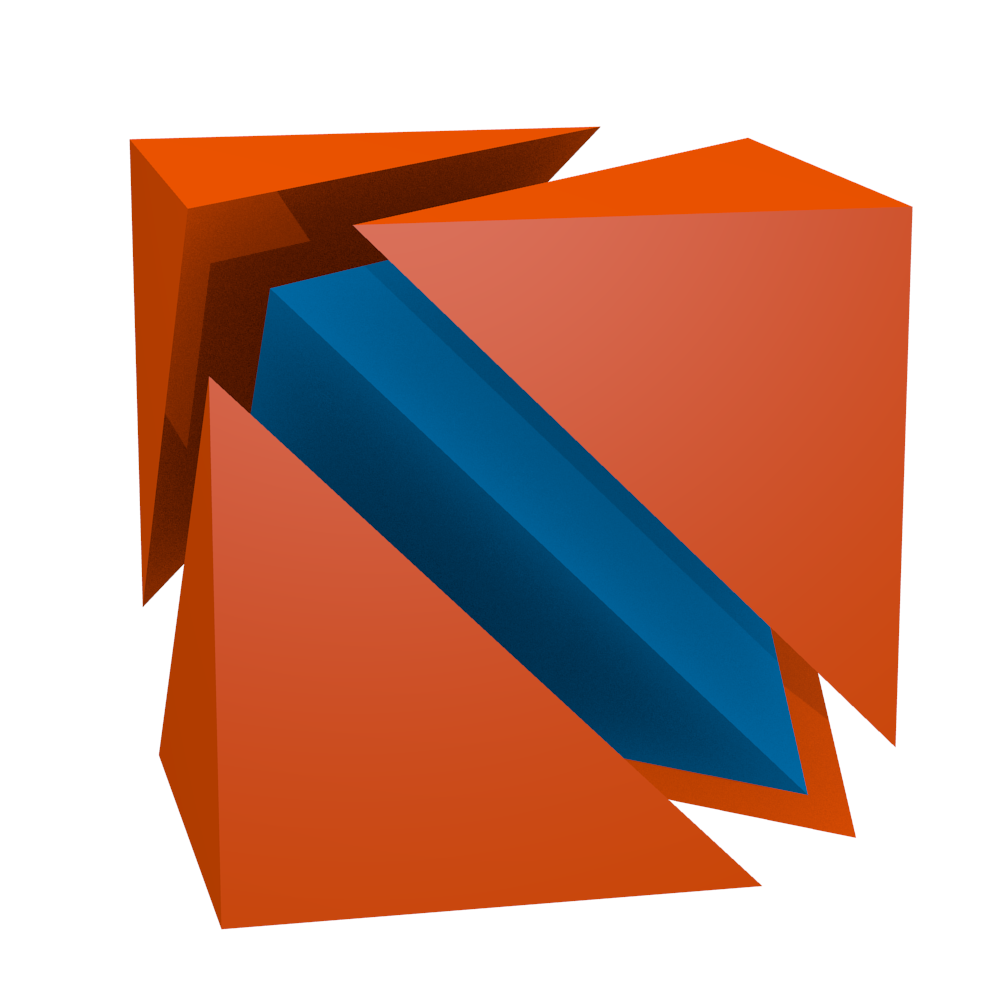
\includegraphics[width=0.4\textwidth]{images/fracture/hexahedron_to_tetrahedra.png}
%     \caption{
%         Illustration of how to divide a hexahedron into five tetraheda.
%         \label{fig:hex_to_tetra}
%     }
% \end{figure}
% 
% \begin{figure}
%     \centering
%     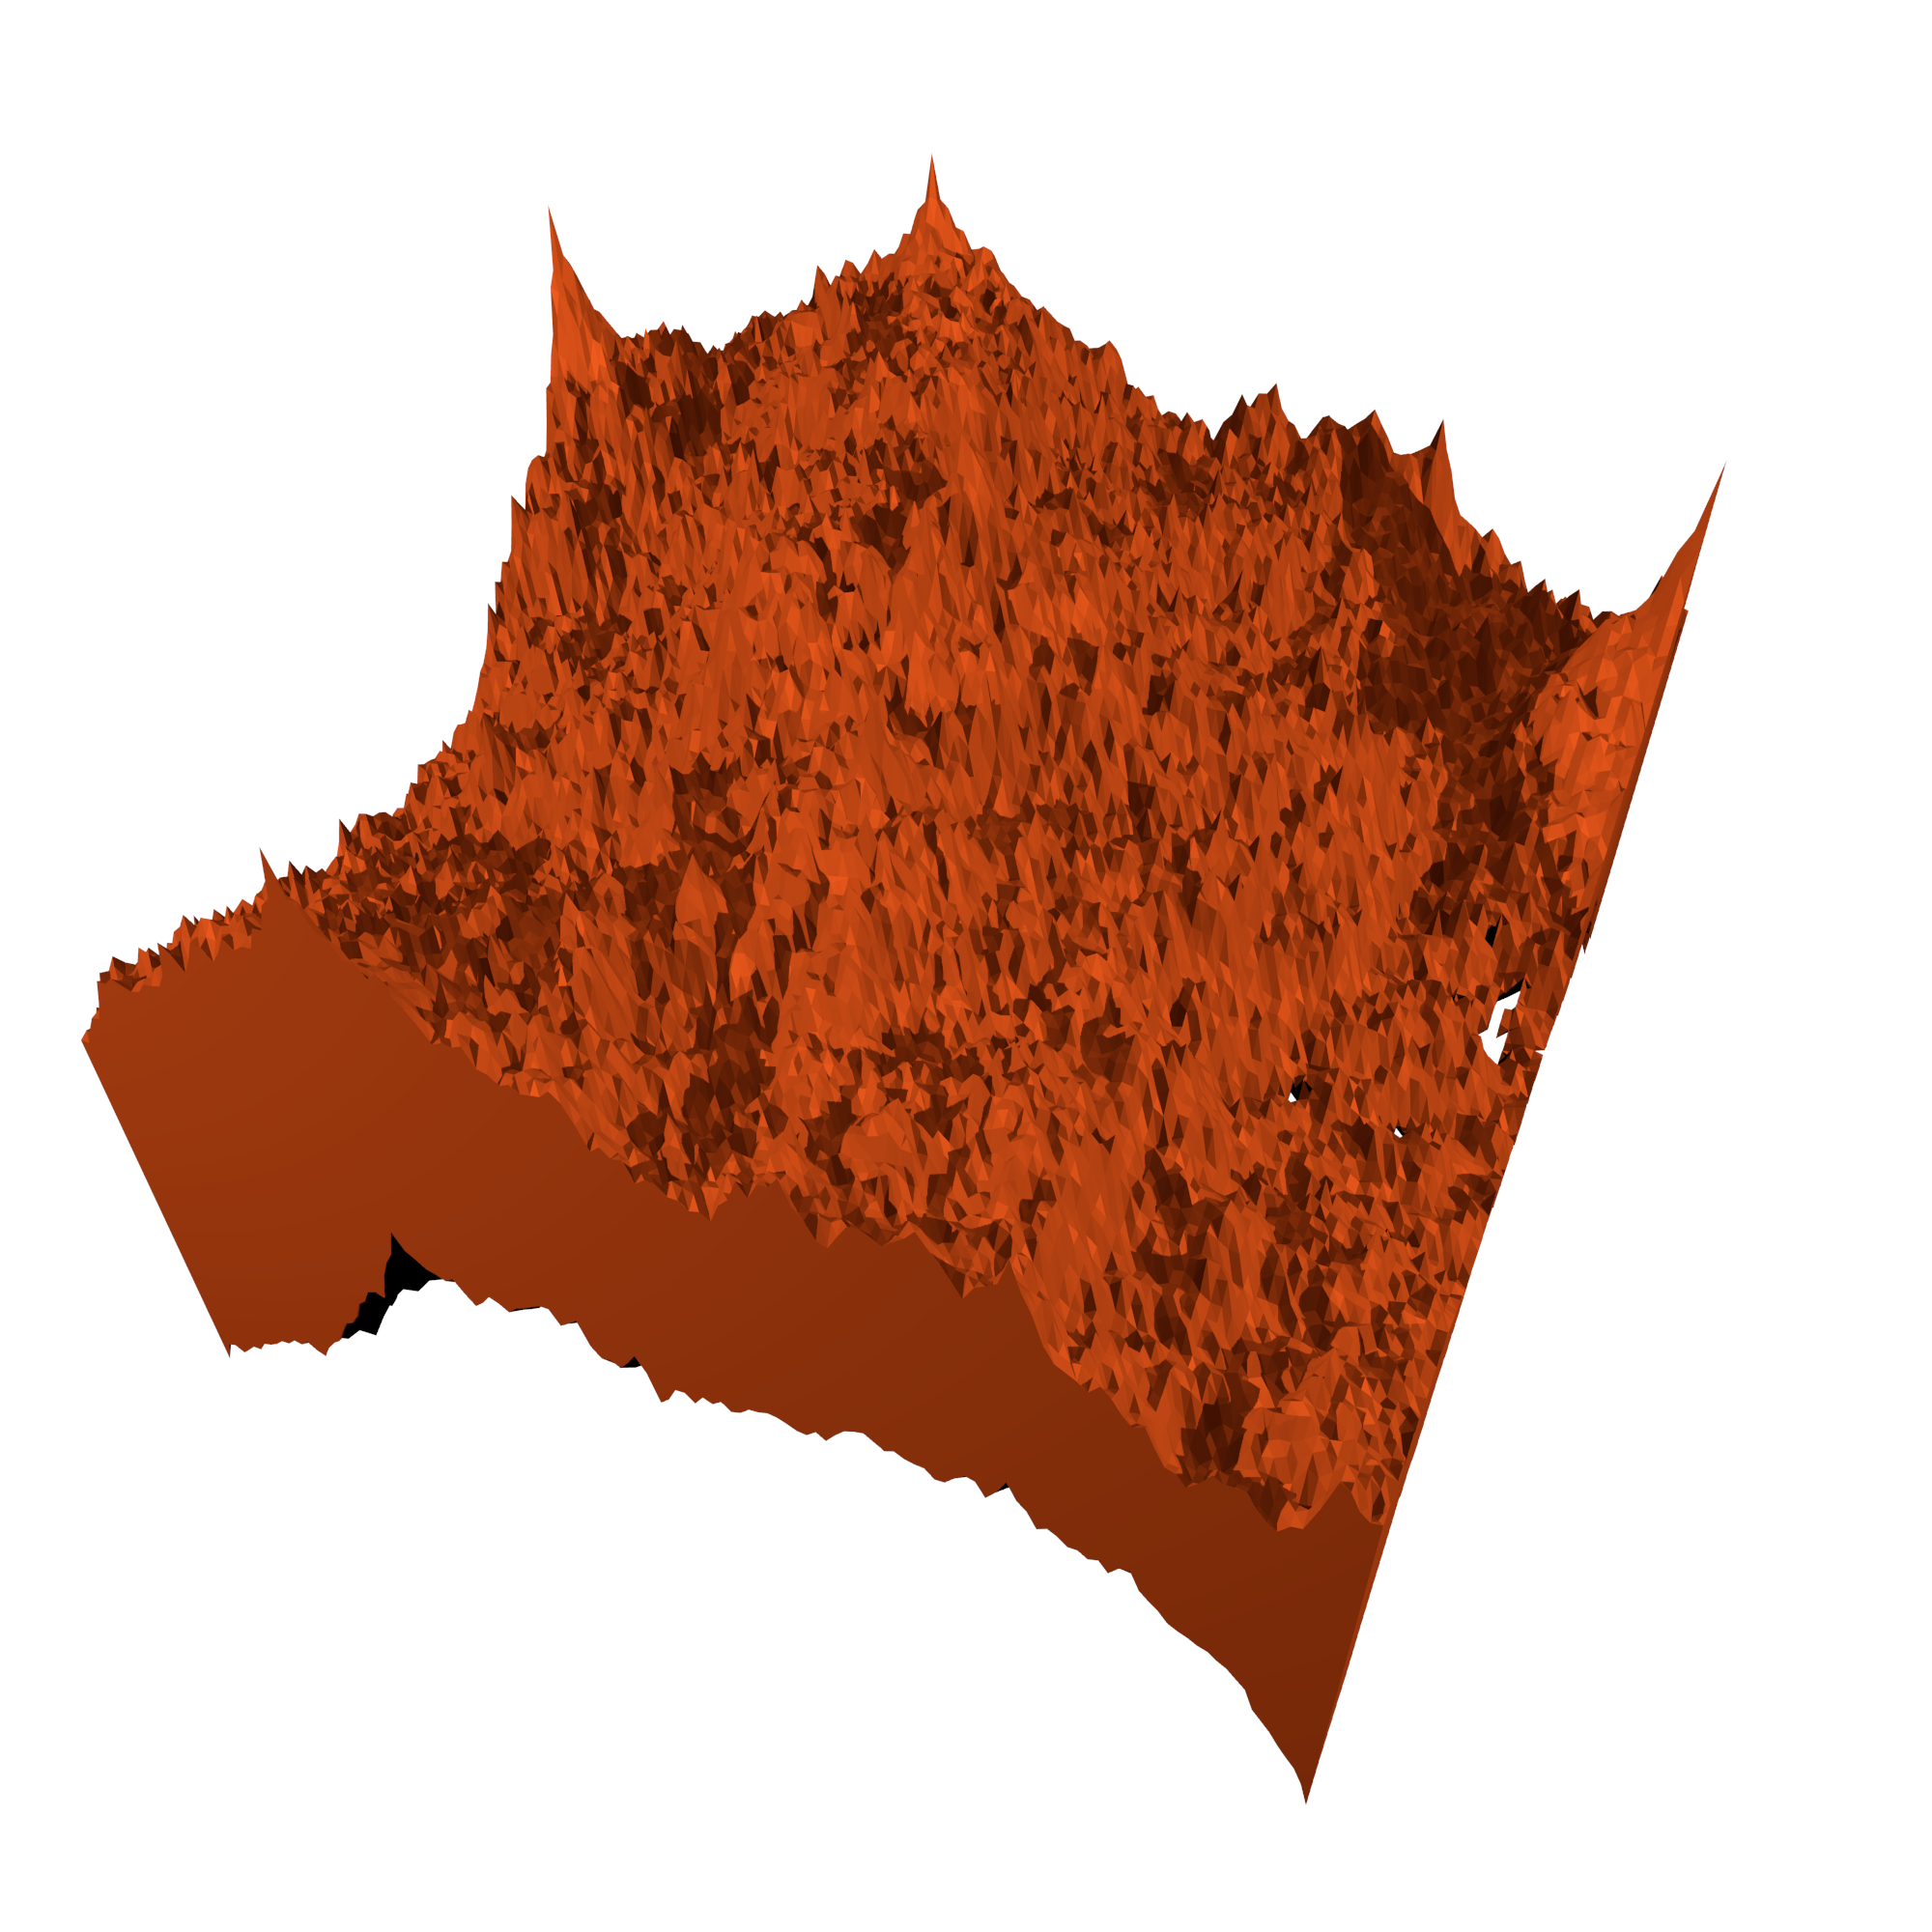
\includegraphics[width=0.6\textwidth]{images/fracture/fracture.png}
%     \caption{
%         A model of a fracture.
%         \label{fig:fracture_model}
%     }
% \end{figure}

\begin{figure}
    \centering
    \begin{subfigure}[b]{0.35\textwidth}
        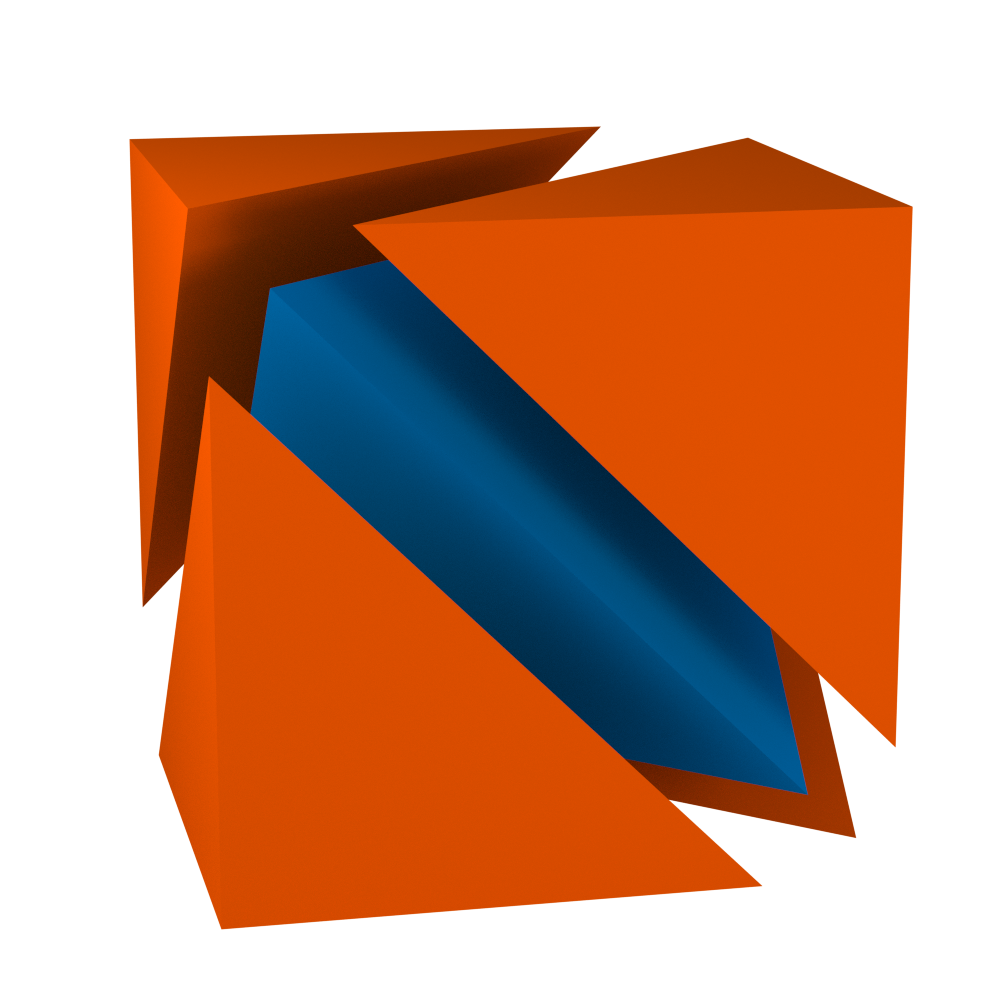
\includegraphics[width=\textwidth]{images/fracture/hexahedron_to_tetrahedra01_cycles_n200.png}
        \caption{Illustration of how to divide a convex hexahedron into five tetraheda.}
        \label{fig:hex_to_tetra}
    \end{subfigure}
    \hspace{5mm}
    \begin{subfigure}[b]{0.55\textwidth}
        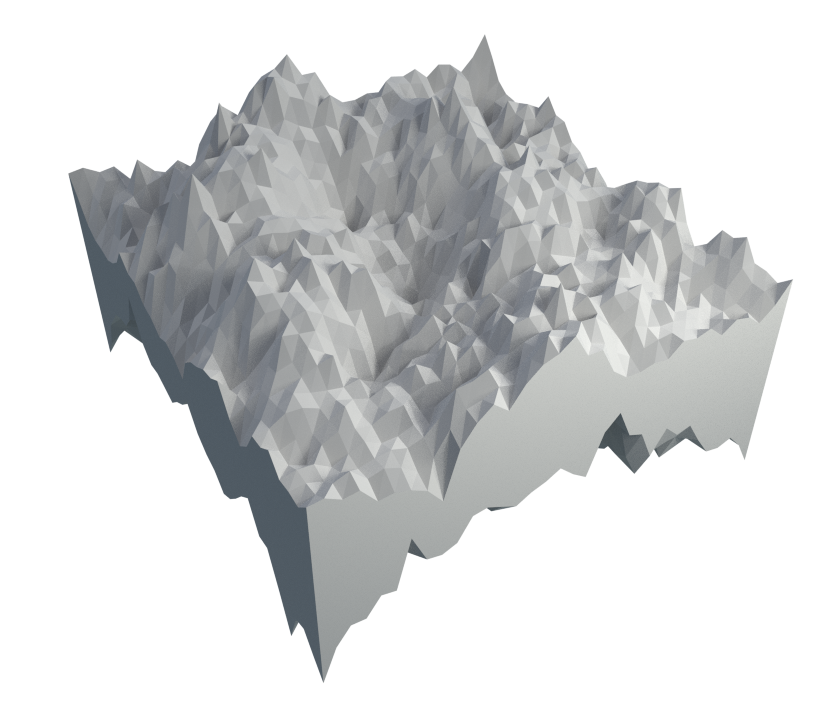
\includegraphics[width=\textwidth]{images/fracture/fracture05_n200.png}
%         \includegraphics[width=\textwidth]{images/fracture/large_fracture04_300dpi_w20cm}
        \caption{A random fracture made from two periodic heightmaps.}
        \label{fig:fracture_model}
    \end{subfigure}
\end{figure}

\subsubsection{Finding a point inside a tetrahedron}
A tetrahedron consists of four points $\bvec a$, $\bvec b$, $\bvec c$, and $\bvec d$, and four faces spanned by the four possible combinations of the four points. For a face spanned by the points $\bvec a$, $\bvec b$, and $\bvec c$ we can find if a point $\bvec P$ is on the same side of the face as the point $\bvec d$ (the point not used to construct the face) by doing some geometry. We find the normal vector to the surface $\bvec n$ by the cross product 
\begin{align*}
    \bvec n = (\bvec a-\bvec c)(\bvec b-\bvec c).
\end{align*}
We know that the sign of the dot product between this normal vector and another vector going from the plane to a point will give us information about which side of the plane the point is. This means that if two points $\bvec p_1$ and $\bvec p_2$ are on the side of the plane, the dot product between the normal vector and the two vectors
\begin{align*}
    (\bvec p_i - \bvec k),
\end{align*}
where $\bvec k$ is any point in the plane, should have the same sign. So we find the sign of dot products
\begin{align*}
    &\text{sgn}\big(\bvec n\cdot(\bvec P - \bvec k)\big), \\
    &\text{sgn}\big(\bvec n\cdot(\bvec d - \bvec k)\big),
\end{align*}
and if the sign of these dot products is the same, we know that the point $\bvec P$ is on the same side of the face as the point $\bvec d$. We now see that if we do this for all four faces of the tetrahedra, we know that the point $\bvec P$ is inside the tetrahedra if the signs of all pairs of dot products are equal.

% Calculating wether a point is inside a tetrahedron can be reduced to comparing the sign of five different matrix determinants. If we have a point $P = (x,y,z)$ and the four vertices of the tetrahedron are $(x_i, y_i, z_i)$ for $i\in \{1,2,3,4\}$, we can find if the point is inside the tetrahedron by checking if the the following five matrix determinants have the same sign
% \begin{align*}
%     &\begin{vmatrix}
%         x_1 & y_1 & z_1 & 1 \\
%         x_2 & y_2 & z_2 & 1 \\
%         x_3 & y_3 & z_3 & 1 \\
%         x_4 & y_4 & z_4 & 1
%     \end{vmatrix},&
%     &\begin{vmatrix}
%         x & y & z & 1 \\
%         x_2 & y_2 & z_2 & 1 \\
%         x_3 & y_3 & z_3 & 1 \\
%         x_4 & y_4 & z_4 & 1
%     \end{vmatrix},&
%     &\begin{vmatrix}
%         x_1 & y_1 & z_1 & 1 \\
%         x & y & z & 1 \\
%         x_3 & y_3 & z_3 & 1 \\
%         x_4 & y_4 & z_4 & 1
%     \end{vmatrix},&
%     \\
% %     \vspace{5mm}
%     \\
%     &\begin{vmatrix}
%         x_1 & y_1 & z_1 & 1 \\
%         x_2 & y_2 & z_2 & 1 \\
%         x & y & z & 1 \\
%         x_4 & y_4 & z_4 & 1
%     \end{vmatrix},&
%     &\begin{vmatrix}
%         x_1 & y_1 & z_1 & 1 \\
%         x_2 & y_2 & z_2 & 1 \\
%         x_3 & y_3 & z_3 & 1 \\
%         x & y & z & 1
%     \end{vmatrix}.&
% \end{align*}
